%Physical principles

\section{Physical Principles}
\subsection{Standard Model}
\begin{figure}[hb]
	\centering
	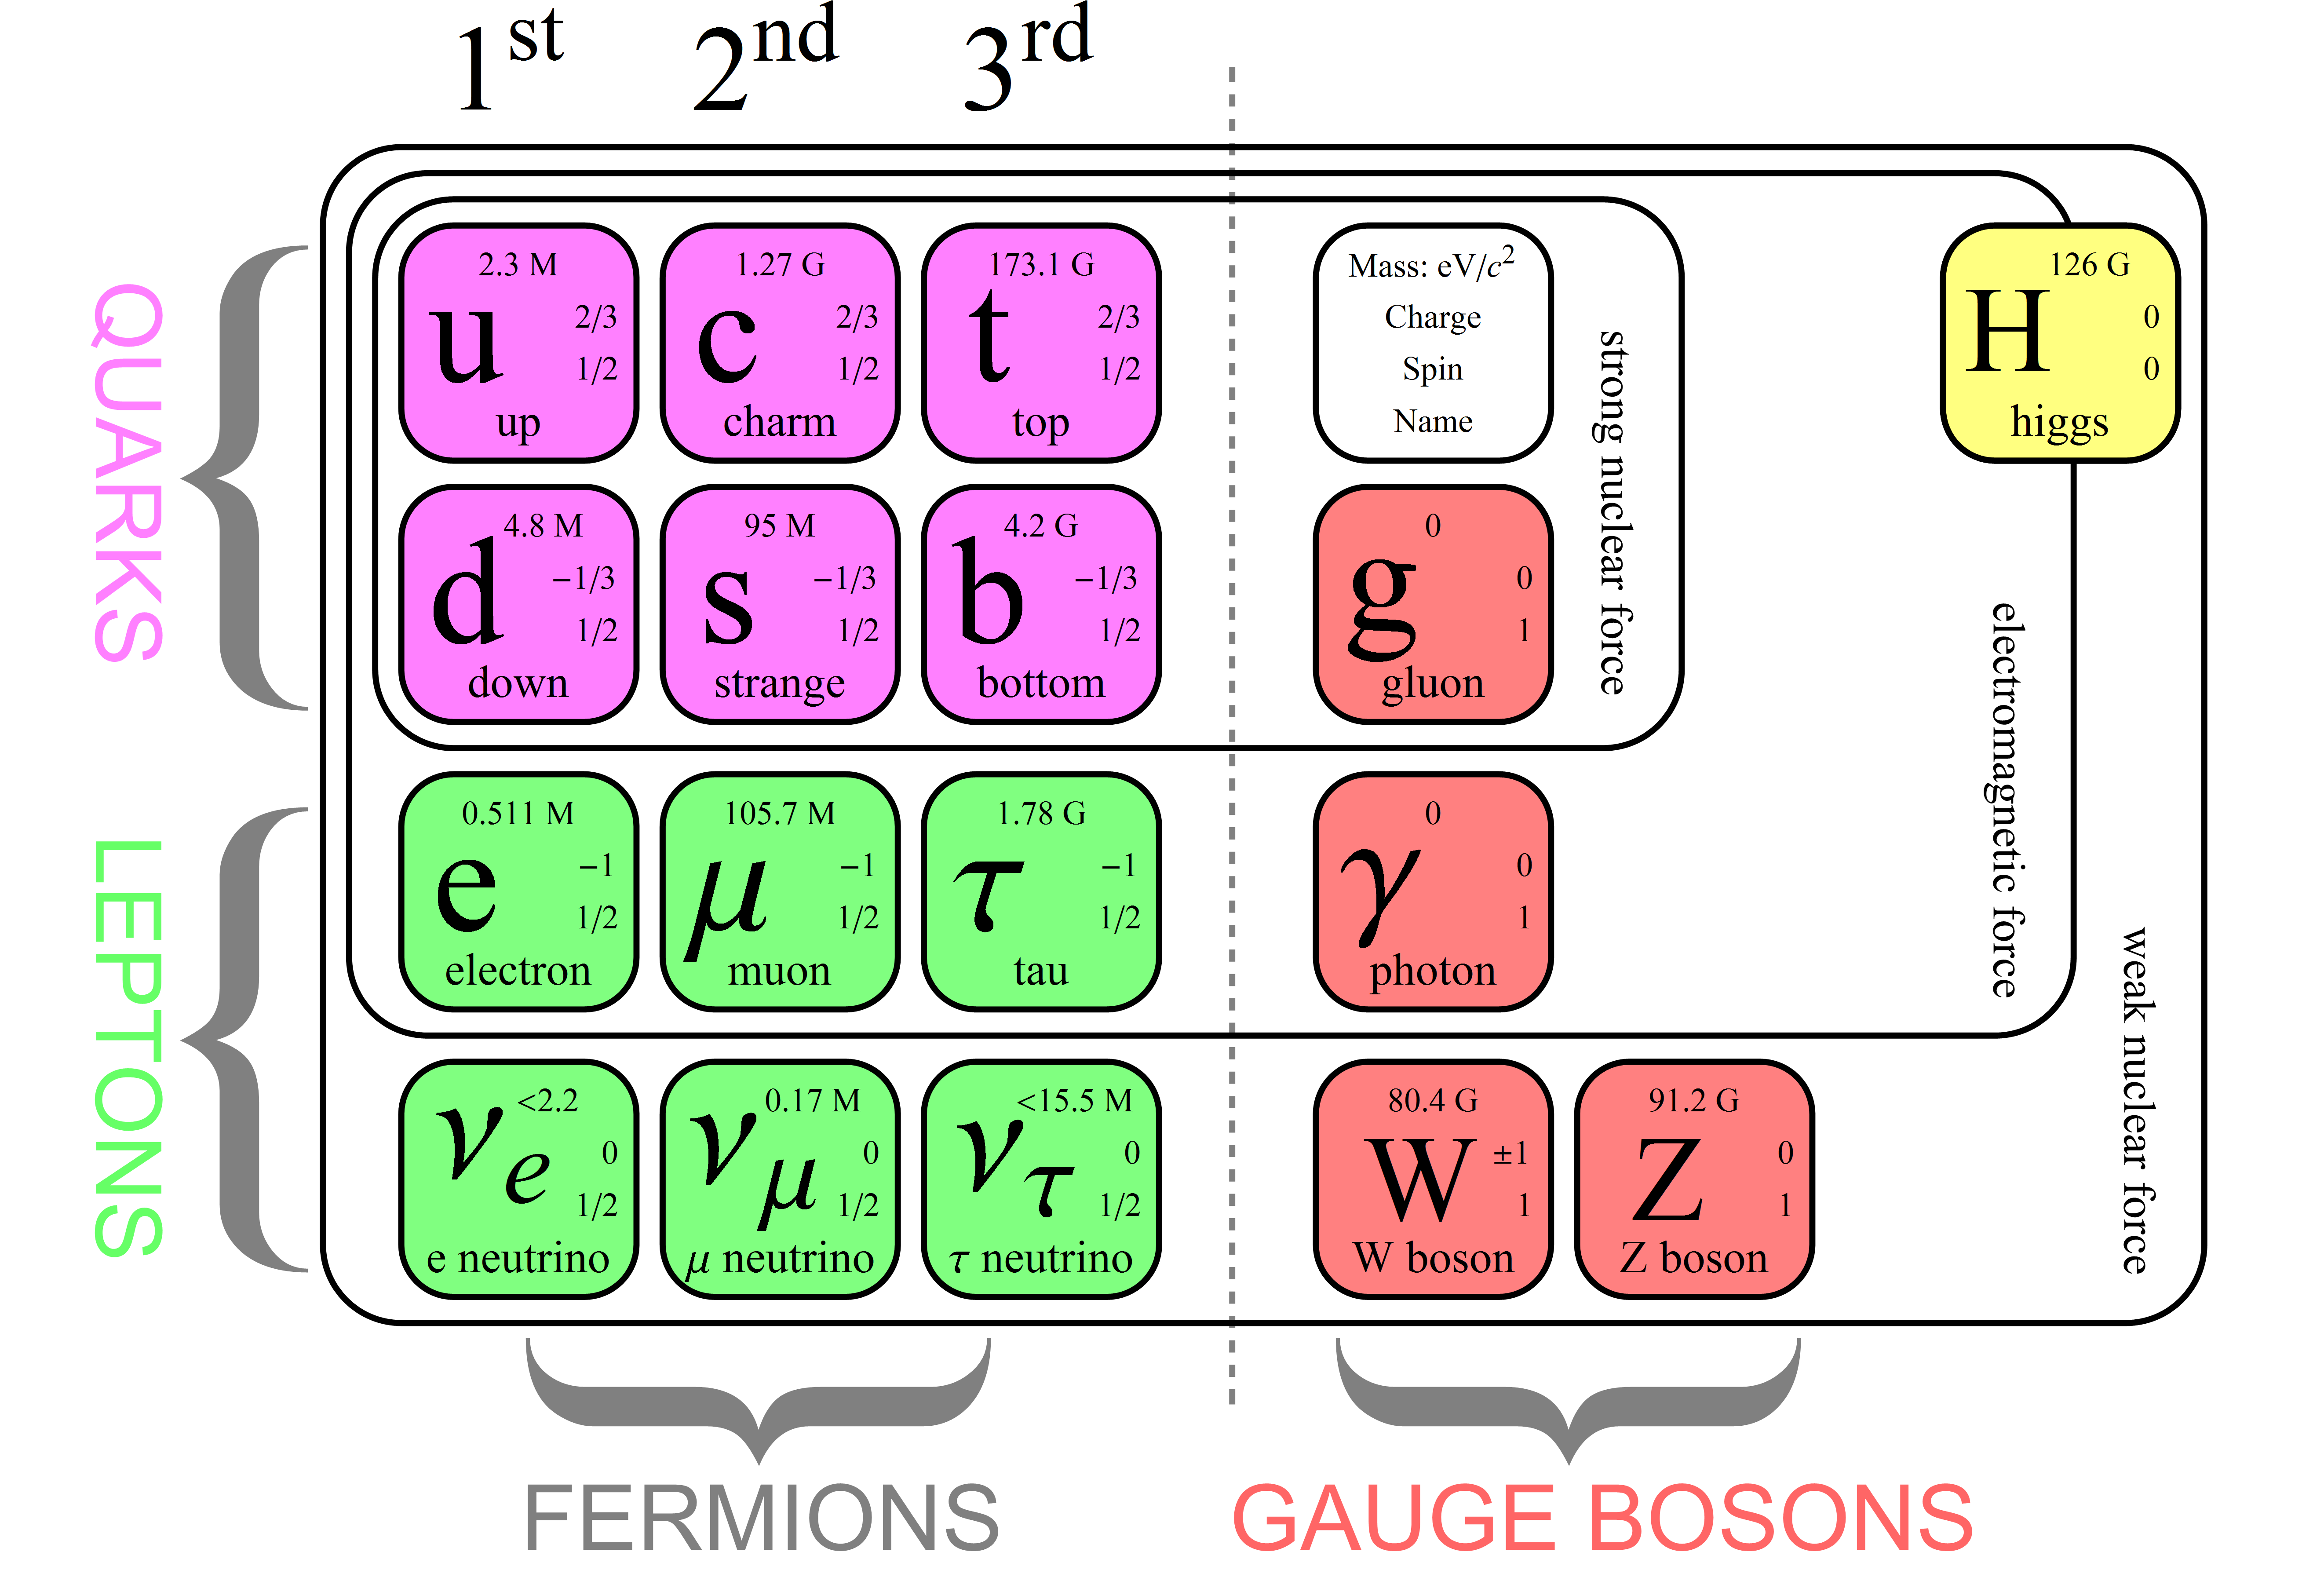
\includegraphics[scale=0.4]{graphics/SM1.png}
	\caption[Standard Model]{Fundamental particles in the Standard Model\cite{uni zuerich}} 
	\label{fig:principles:Standard_Model_of_Elementary_Particles}
\end{figure}

Figure~\ref{fig:principles:Standard_Model_of_Elementary_Particles} gives an overview of the fundamental particles in the Standard Model. Quarks and Leptons obey the Pauli exclusion principle and are therefore fermions. Each of those also has a corresponding antiparticle with the same mass but opposite charge. Fundamental interactions are mediated by the Gauge Bosons, namely two particles interact with each other by exchanging said bosons. The original theory stated that fermions and bosons are massless, they gain mass via the Higgs-Kibble mechanism which implies the existence of another particle, the Higgs Boson\cite{muenchen}.

\subsection{Electroweak force and Weinberg Angle}
1967 Glasgow, Salam and Weinberg were able to unify the electromagnetic and weak force. In this model the electroweak interaction is mediated by four Bosons $W^1$, $W^2$, $W^3$ and $B^0$. The Bosons of the Standard Model are then described as a linear combination of those Bosons; two charged states

\begin{equation}
\ket{W^{\pm}}=(1/\sqrt{2}) (\ket{W^1}\mp i\ket{W^2})
\end{equation}

and the photon and $Z^0$ Boson as orthogonal neutral states\cite{Grif}

\begin{equation}
\begin{aligned}
\ket{\gamma} &=  cos(\theta_w)\ket{B^0} + sin(\theta_w) \ket{W^0}\\
\ket{Z^0} &= -sin(\theta_w) \ket{B^0} + cos(\theta_w) \ket{W^0}
\end{aligned}
\end{equation}

The mixing angle $\theta_w$ is called \emph{Weinberg angle}. It is further related to the fine-structure constant  $\alpha$, the Fermi coupling constant $G_F$ and the mass of the $Z^0$ Boson\cite{muenchen}:

\begin{equation}
sin^2(\theta_w)\cdot cos^2(\theta_w) = \frac{\pi\alpha}{\sqrt{2}G_FM_Z^2}
\end{equation}

The mass of the $W^{\pm}$ Bosons can be expressed as:
\begin{equation}
M_W = M_Z~cos(\theta_w)
\end{equation}

In electroweak interaction one distinguishes two forms of coupling, vector (changes sign under parity transformation) and axial vector (does not change sign under parity transformation) coupling. The coupling strengths for a fermion $f$ with the third component of weak isospin $I^f_3$ and the charge $Q_f$ is given by\cite{muenchen}:

\begin{equation}
\begin{aligned}
g_V^f &= I^f_3-2 Q_f sin^2(\theta_w)\\
g_A^f &= I^f_3
\end{aligned}
\label{eq:principles:coupling strengths}
\end{equation}

\subsection{Cross Section and decay width}
The cross section $\sigma$ is a measure for the probability or rate of a reaction during collision of two particles. In this experiment it is related to the Luminosity $L$ of the electron beam and the total Number of reactions $N$:

\begin{equation}
\sigma = \frac{N}{\int L~\text{d}t}
\end{equation}

In those collisions new particles can be created that in turn may decay with a mean life time $T$.
Heisenberg's uncertainty principle relates the mean life with the (total)\emph{decay width}:

\begin{equation}
\hbar=T\cdot\Gamma
\end{equation}

Often the particle can decay through different channels. The probability that a decay takes channel $i$ is called the branching ratio $BR_i$. It can be described with the \emph{partial} decay width $\Gamma_i$:

\begin{equation}
\Gamma = \sum_i \Gamma_i
\end{equation}

The branching ratio is then:

\begin{equation}
BR_i=\frac{\Gamma_i}{\Gamma}
\label{eq:principles:branching ratio}
\end{equation}

\subsection{$e^-e^+$ Interactions}
\label{sec:ee interaction}
\begin{figure}[ht]
	\centering
	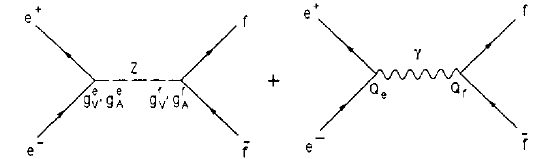
\includegraphics{graphics/annihilation.png}
	\caption[Feynman diagramm: $e^-e^+ \rightarrow f\bar{f} $(s-channel)]{Feynman diagram of the $e^-e^+ \rightarrow f\bar{f}$ in first order, where f is an arbitrary fermion.} 
	\label{fig:principles:annihilation.png}
\end{figure}

The reaction were interested for this experiment is the $e^-e^+\rightarrow\bar{f}$ interaction. Figure \ref{fig:principles:annihilation.png} shows the s-channel: Electron and positron annihilate each other and a $Z^0$ Boson or a photon is produced, which in turn decay to a lepton or a Quark and its corresponding antiparticle (except for the top quark, since the center-of-mass energy is less than the mass of two top quarks). The photon process is repressed at energies close to the Mass of the $Z^0$ Boson\cite{muenchen}.\\%wie stark?
The cross section for the $e^-e^+\rightarrow f\bar{f}$ reaction is a function of the center-of-mass energy, which exhibits a peak at 91.187 GeV caused by the $Z^0$ resonance(s. fig \ref{fig:principles:crosssection}).

\begin{figure}[H]
\centering
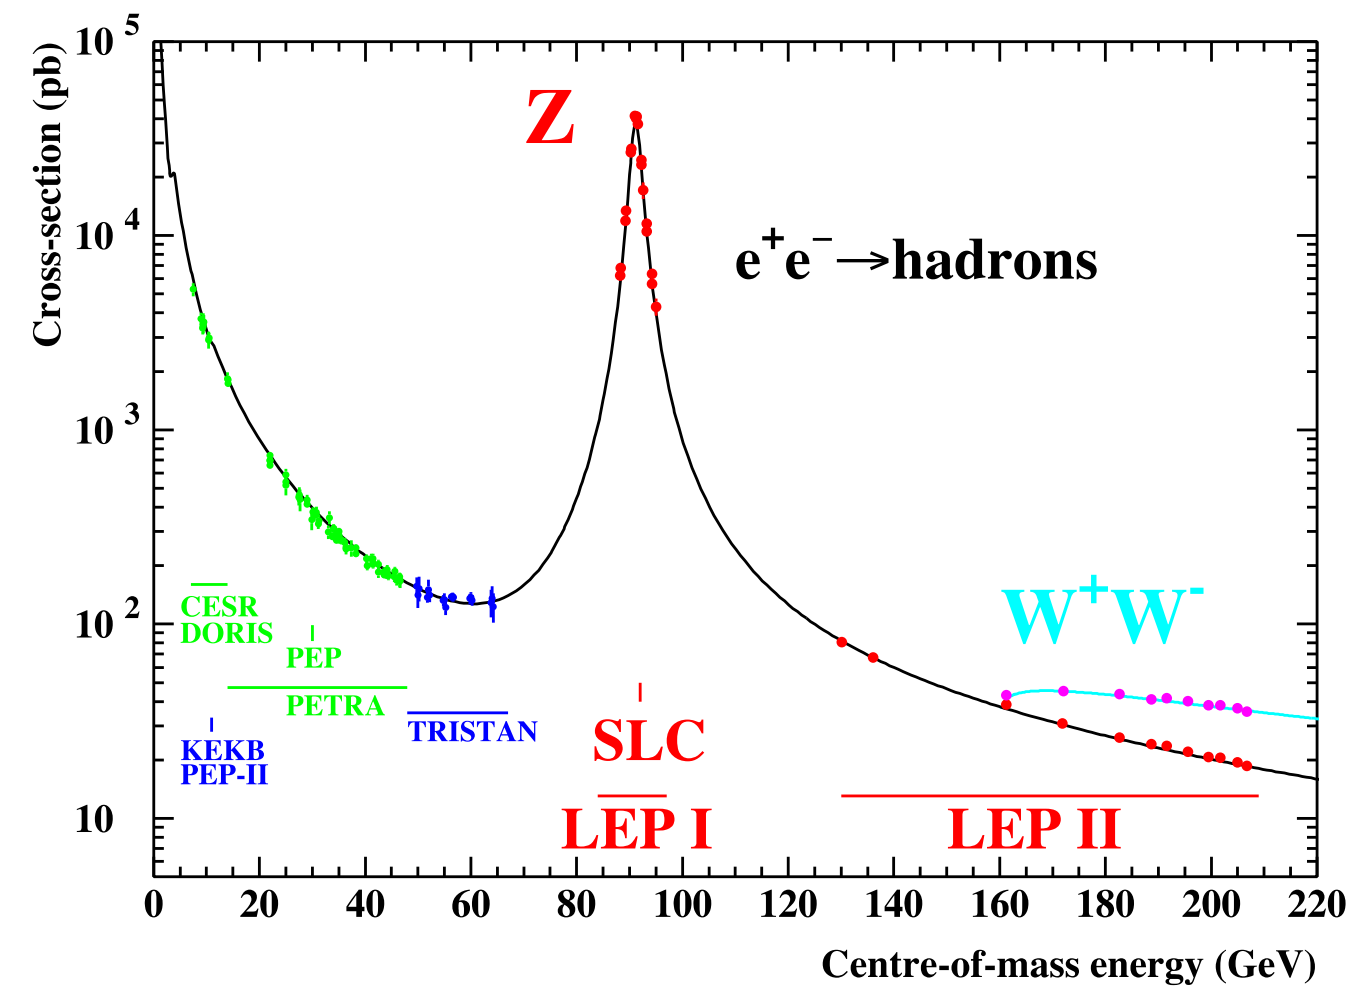
\includegraphics[width=\linewidth]{graphics/crosssection}
\caption[cross section as a function of CMS]{cross section for the $e^+ e^- \rightarrow q \bar{q}$ reaction as a function of the center-of-mass energy. The peak at 91.187 GeV is the $Z^0$ resonance peak \cite{jakobs}}
\label{fig:principles:crosssection}
\end{figure}

 Neglecting the fermion masses and at energies close to the resonance this function can be described with a Breit-Wigner curve\footnote{For a table of theoretical decay widths and cross section and their calculation s. appendix}\cite{muenchen}:
 
\begin{equation}
\sigma_f(s) = \frac{12\pi}{M_Z^2} \frac{s\Gamma_e\Gamma_f}{(s-M_Z^2)^2+s^2\Gamma_Z^2/M_Z^2}
\label{eq:principles:breitwigner}
\end{equation}

Where $\sqrt{s}$ is the center-of-mass energy, $M_Z$ the $Z_0$ mass, $\Gamma_Z$ the total \emph{decay width}, $\Gamma_e$ the partial decay width for electrons and $\Gamma_f$ the partial decay width.
\begin{figure}[H]
	\centering
	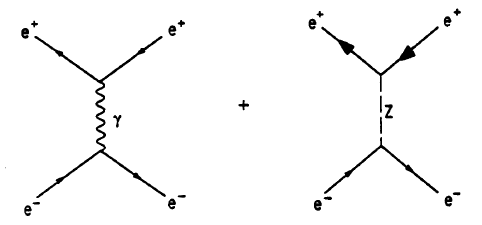
\includegraphics{graphics/BhabbaStreuung.png}
	\caption[Feynman diagram: Bhabha scattering]{Feynman diagrams of the $e^-e^+ \rightarrow e^-e^+$ scattering (t-channel)\cite{muenchen}}
	\label{fig:principles:BhabbaStreuung.png}
\end{figure}
Figure \ref{fig:principles:BhabbaStreuung.png} shows the t-channel of the  $e^-e^+ \rightarrow e^-e^+$ reaction. The partial cross sections for s- and t-channel differ in their relation to the polar angle $\theta$ (with the positron beam axis as z-axis) of the scatter electron and positron\cite{staatsex}:
\begin{equation}
\frac{d\sigma_s}{d\Omega} \propto (1+cos^2(\theta)),\qquad\frac{d\sigma_t}{d\Omega}t \propto (1-cos(\theta))^{-2}
\label{eq:principles:s-t-channel}
\end{equation}
\subsection{radiation correction}
\label{sec:principles:radiation correction}
The Feynman diagrams in the previous chapter were only first order. Neglecting higher orders (Born approximation) does not yield accurate predictions\cite{muenchen}. Three different corrections have to made: the photonic, the non-photonic and the Quantum chromodynamic (QCD) correction.
\begin{figure}[H]
\centering
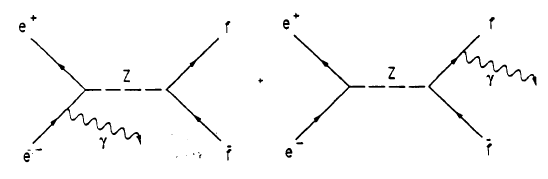
\includegraphics{graphics/Bremsstrahlungskorrektur}
\caption[Feynman diagram: initial and final state radiation]{Feynman diagram for initial state (left) and final state radiation (right)\cite{muenchen}}
\label{fig:principles:Bremsstrahlungskorrektur}
\end{figure}
During initial and final state radiation (see fig. \ref{fig:principles:Bremsstrahlungskorrektur}) the a photon is emitted. The energy this photon carries is not available for $Z^0$ production. Therefore at center-of-mass energies $\sqrt{s}\leq M_Z$, this process decreases the cross section and	for energies $\sqrt{s} > M_Z$ the cross section is increased.\\
Non photonic processes have the same final state as the first order process, but as seen in figure \ref{fig:principles:vertexschleifen} the interaction is complicated by vertex loops. Those additional Feynman diagrams have to be accounted for in the cross section.\\
\begin{figure}[H]
	\centering
	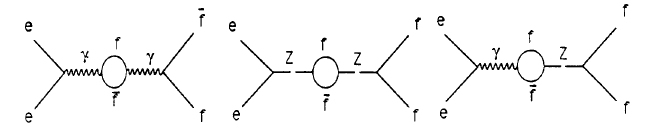
\includegraphics[width=1.0\linewidth]{graphics/vertexschleifen}
	\caption[Feynman diagramm: virtual radiation]{Feynman diagram for virtual radiation correction. The final state is the same as in figure \ref{fig:principles:annihilation.png}, but the path is complicated by vertex loops. \cite{muenchen}}
	\label{fig:principles:vertexschleifen}
\end{figure}
If the produced fermions are quarks,  an additional correction has to be made to account for gluon radiation(fig \ref{fig:principles:QCDkorrektur}) of the strong interaction.
\begin{figure}[H]
\centering
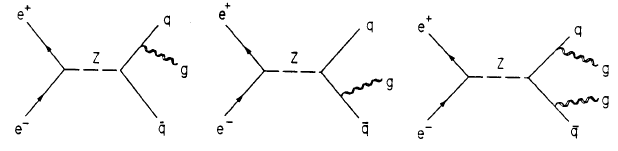
\includegraphics[width=1.0\linewidth]{graphics/QCDkorrektur}
\caption[Feynman daigram: gluon radiation]{Feynman diagram of gluon radiation. In contrast to leptons, quarks interact not only electroweak but also via the strong force and can radiate gluons.\cite{muenchen}}
\label{fig:principles:QCDkorrektur}
\end{figure}
\subsection{Forwards-backwards Asymmetry}
The for equation \ref{eq:principles:s-t-channel} introduced spherical coordinates allow the definition of cross sections for the forward and backwards hemisphere:
\begin{equation}
\sigma_f=\int_{0}^{1}\frac{\text{d}\sigma}{\text{d}cos(\theta)}~\text{d}cos(\theta) \\
\sigma_b=\int_{-1}^{0}\frac{\text{d}\sigma}{\text{d}cos(\theta)}~\text{d}cos(\theta)
\label{eq:principles:fbintegral}
\end{equation}
The forwards backwards asymmetry is then defined as:
\begin{equation}
A_{fb}=\frac{\sigma_f-\sigma_b}{\sigma_f+\sigma_b}
\label{eq:principles:asymmetry definition}
\end{equation}
At the resonance peak the difference in coupling strength for vector and axial vector coupling (s. eq.\ref{eq:principles:coupling strengths}) causes an asymmetry as defined above. For leptons it can be expressed as:
\begin{equation}
A_{fb}^{\ell,peak}\approx 3 \left ( \frac{g^{\ell}_V}{g^{\ell}_A} \right )^2=3\cdot (1-4 sin^2(\theta_w))
\label{eq:principles:asymmetry weinberg angle}
\end{equation}